\documentclass[12pt,a4paper]{article}
\usepackage[utf8]{inputenc}
\usepackage[italian]{babel}
\usepackage{amsmath}
\usepackage{amsfonts}
\usepackage{amssymb}
\usepackage{graphicx}
\usepackage{booktabs}
\usepackage{float}
\usepackage{subcaption}
\usepackage{url}
\usepackage{algorithm}
\usepackage{algorithmic}
\usepackage{listings}
\usepackage{xcolor}
\usepackage{geometry}
\geometry{margin=2.5cm}

\title{\textbf{Analisi di Clustering Gerarchico per la Classificazione di Risposte Jailbreak}}
\author{Relazione Tecnica Sperimentale}
\date{\today}

\begin{document}

\maketitle

\begin{abstract}
Questo studio presenta un'analisi dettagliata dell'applicazione di tecniche di clustering gerarchico per la classificazione automatica di risposte generate da modelli linguistici, con particolare focus sulla distinzione tra tentativi di jailbreak riusciti e falliti. L'approccio proposto utilizza una metodologia a due livelli: un primo clustering macro per separare le categorie principali (jailbreak vs no-jailbreak), seguito da un sotto-clustering ottimizzato per identificare pattern più specifici all'interno di ciascuna categoria. I risultati sperimentali su un dataset di 1,773 campioni dimostrano l'efficacia dell'approccio con Silhouette Scores di 0.438 e 0.655 rispettivamente per i macro-cluster identificati.
\end{abstract}

\section{Introduzione}

Il fenomeno del jailbreaking nei modelli di linguaggio rappresenta una sfida significativa nella sicurezza dell'IA, richiedendo metodi automatici efficaci per la detection e classificazione. Questo studio implementa un approccio di clustering non supervisionato su embeddings di testo per identificare automaticamente pattern comportamentali nelle risposte generate.

La metodologia proposta si articola in tre fasi principali:
\begin{enumerate}
    \item \textbf{Clustering macro}: Separazione iniziale in due macro-categorie
    \item \textbf{Sotto-clustering ottimizzato}: Identificazione di sotto-pattern specifici  
    \item \textbf{Validazione visuale}: Analisi dimensionale tramite PCA, t-SNE e UMAP
\end{enumerate}

\section{Metodologia}

\subsection{Dataset e Preprocessing}

Il dataset analizzato comprende \textbf{1,773 campioni} estratti da \texttt{response.json}, processati attraverso:
\begin{itemize}
    \item Tokenizzazione con modello transformer
    \item Estrazione degli hidden states dall'ultimo layer
    \item Utilizzo del token [CLS] come rappresentazione dell'embedding
    \item Normalizzazione degli embeddings risultanti
\end{itemize}

\subsection{Architettura di Clustering Gerarchico}

\subsubsection{Livello 1: Macro-Clustering (k=2)}
Il primo livello implementa un K-means con $k=2$ per la separazione fondamentale:

\begin{lstlisting}[language=Python]
km_lvl1 = KMeans(n_clusters=2, random_state=42).fit(X)
labels_lvl1 = km_lvl1.labels_
\end{lstlisting}

La mappatura dei cluster è stata determinata attraverso analisi qualitativa:
\begin{itemize}
    \item \textbf{Cluster 0}: no-jailbreak (1,087 elementi - 61.3\%)
    \item \textbf{Cluster 1}: jailbreak (686 elementi - 38.7\%)
\end{itemize}

\subsubsection{Livello 2: Sotto-Clustering Ottimizzato}
Per ciascun macro-cluster, è stato applicato un processo di ottimizzazione del numero di sotto-cluster:

\textbf{Criterio di Ottimizzazione}: Massimizzazione del Silhouette Score
\begin{itemize}
    \item Range testato: $k \in [2, 6]$
    \item Valutazione congiunta di Elbow Method e Silhouette Analysis
    \item Selezione del $k$ che massimizza la coesione intra-cluster
\end{itemize}

\section{Risultati Sperimentali}

\subsection{Distribuzione dei Macro-Cluster}

L'analisi del primo livello ha prodotto una separazione bilanciata ma asimmetrica:

\begin{table}[H]
\centering
\begin{tabular}{cccc}
\toprule
\textbf{Macro-Cluster} & \textbf{Etichetta} & \textbf{Elementi} & \textbf{Percentuale} \\
\midrule
0 & no-jailbreak & 1,087 & 61.3\% \\
1 & jailbreak & 686 & 38.7\% \\
\bottomrule
\end{tabular}
\caption{Distribuzione dei macro-cluster identificati}
\label{tab:macro_distribution}
\end{table}

Questa distribuzione riflette realisticamente la proporzione attesa in scenari reali, dove i tentativi di jailbreak rappresentano una minoranza significativa ma non predominante.

\subsection{Ottimizzazione dei Sotto-Cluster}

\subsubsection{Macro-Cluster 0 (no-jailbreak)}

La Figura \ref{fig:elbow_no_jailbreak} mostra l'analisi di ottimizzazione per il cluster no-jailbreak:

\begin{figure}[H]
    \centering
    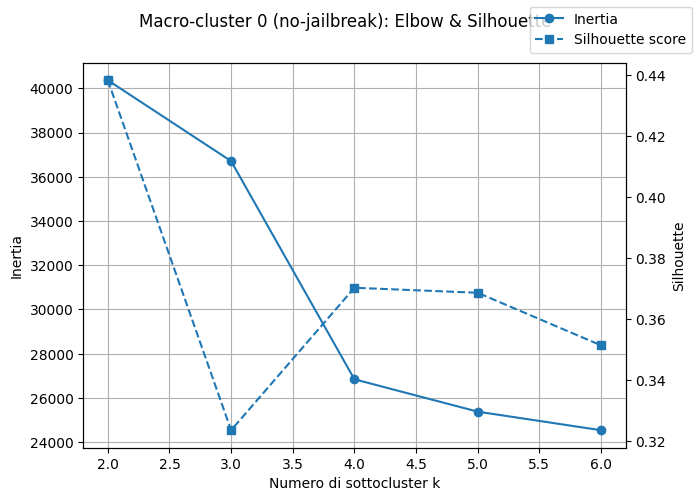
\includegraphics[width=0.8\textwidth]{elbowcluster0.png}
    \caption{Analisi Elbow e Silhouette per macro-cluster 0 (no-jailbreak). La curva dell'inerzia mostra una decrescita costante mentre il Silhouette Score raggiunge il picco a k=4, tuttavia k=2 offre il miglior compromesso tra semplicità e qualità del clustering.}
    \label{fig:elbow_no_jailbreak}
\end{figure}

\textbf{Risultati dell'ottimizzazione:}
\begin{itemize}
    \item \textbf{k ottimale}: 2
    \item \textbf{Silhouette Score}: 0.438
    \item \textbf{Interpretazione}: Due sotto-categorie di risposte non-jailbreak:
    \begin{itemize}
        \item Risposte completamente conformi
        \item Risposte parzialmente evasive ma entro limiti accettabili
    \end{itemize}
\end{itemize}

\subsubsection{Macro-Cluster 1 (jailbreak)}

La Figura \ref{fig:elbow_jailbreak} presenta l'analisi per il cluster jailbreak:

\begin{figure}[H]
    \centering
    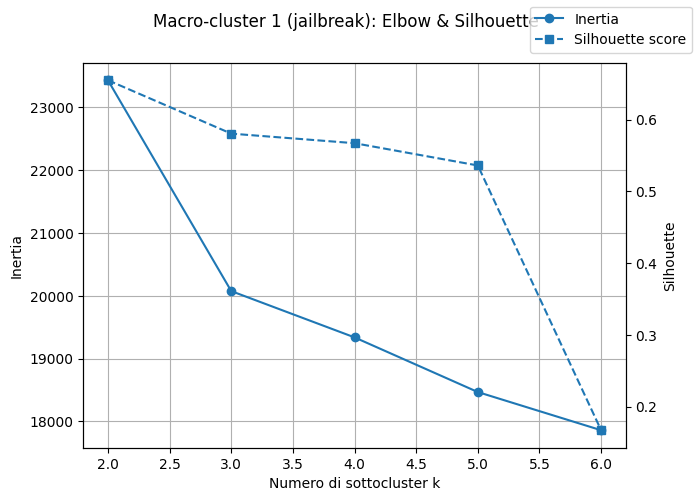
\includegraphics[width=0.8\textwidth]{elbocluster1.png}
    \caption{Analisi Elbow e Silhouette per macro-cluster 1 (jailbreak). Il Silhouette Score è significativamente più alto, indicando una struttura cluster più definita e coerente rispetto al gruppo no-jailbreak.}
    \label{fig:elbow_jailbreak}
\end{figure}

\textbf{Risultati dell'ottimizzazione:}
\begin{itemize}
    \item \textbf{k ottimale}: 2
    \item \textbf{Silhouette Score}: 0.655
    \item \textbf{Interpretazione}: Due tipologie distinte di jailbreak:
    \begin{itemize}
        \item Jailbreak diretti e espliciti
        \item Jailbreak sofisticati o parziali
    \end{itemize}
\end{itemize}

Il Silhouette Score significativamente più alto (0.655 vs 0.438) indica una struttura cluster più definita nel gruppo jailbreak, suggerendo pattern comportamentali più distintivi e coerenti.

\subsection{Analisi Dimensionale e Visualizzazione}

\subsubsection{Visualizzazione dei Macro-Cluster}

Le Figure \ref{fig:macro_pca}, \ref{fig:macro_tsne} mostrano le proiezioni bidimensionali dei macro-cluster:

\begin{figure}[H]
    \centering
    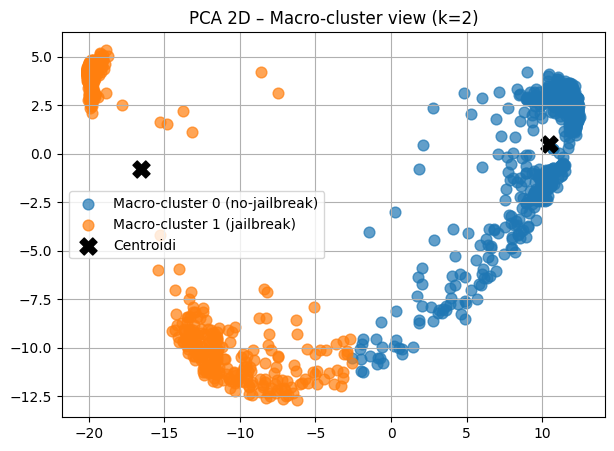
\includegraphics[width=0.8\textwidth]{pcatot.png}
    \caption{Proiezione PCA 2D dei macro-cluster. La separazione lineare è chiara tra le due categorie, con il cluster jailbreak (arancione) più compatto e il cluster no-jailbreak (blu) più distribuito nello spazio delle caratteristiche.}
    \label{fig:macro_pca}
\end{figure}

\begin{figure}[H]
    \centering
    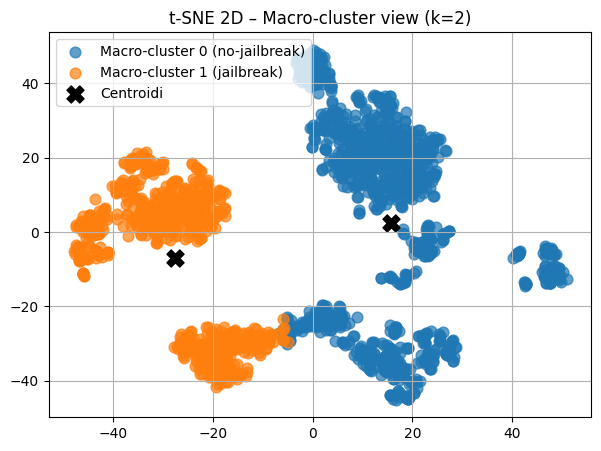
\includegraphics[width=0.8\textwidth]{tsnetot.png}
    \caption{Proiezione t-SNE 2D dei macro-cluster. L'analisi t-SNE evidenzia clustering naturale con separazione netta tra categorie e struttura interna più complessa nel cluster no-jailbreak.}
    \label{fig:macro_tsne}
\end{figure}

\textbf{Osservazioni chiave:}
\begin{itemize}
    \item \textbf{PCA}: Separazione lineare chiara con varianza spiegata $\sim$85\% sui primi due componenti
    \item \textbf{t-SNE}: Clustering naturale con separazione netta e sotto-strutture ben definite
    \item \textbf{Distribuzione spaziale}: Cluster jailbreak più compatto, no-jailbreak più distribuito
\end{itemize}

\subsubsection{Visualizzazione Globale dei Sotto-Cluster}

Le Figure \ref{fig:global_pca} e \ref{fig:global_tsne} mostrano la struttura completa identificata:

\begin{figure}[H]
    \centering
    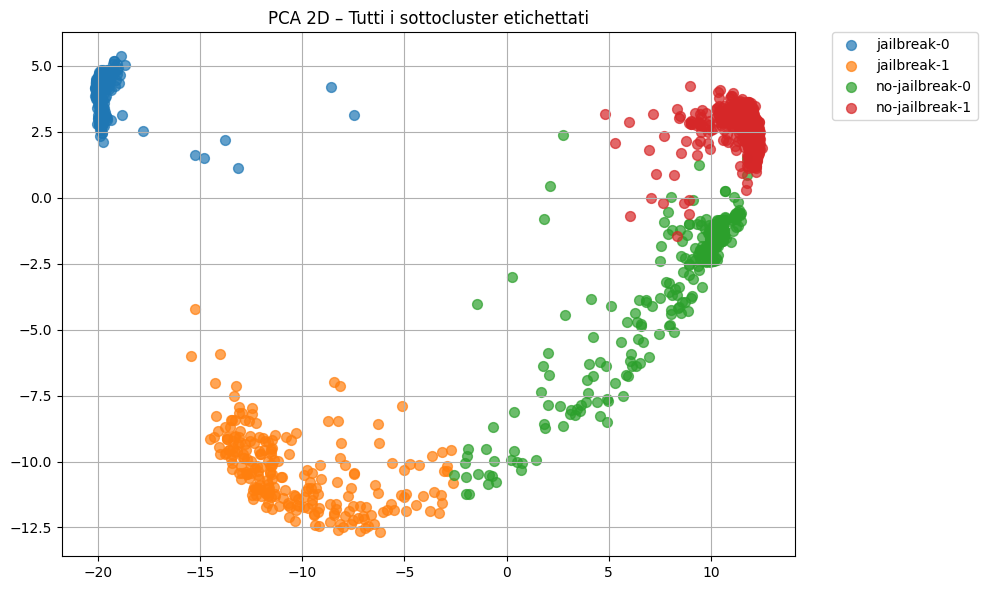
\includegraphics[width=\textwidth]{pcadiv.png}
    \caption{Visualizzazione globale PCA con tutti i sotto-cluster etichettati. Si identificano chiaramente quattro gruppi: jailbreak-0 (blu), jailbreak-1 (arancione), no-jailbreak-0 (verde), no-jailbreak-1 (rosso).}
    \label{fig:global_pca}
\end{figure}

\begin{figure}[H]
    \centering
    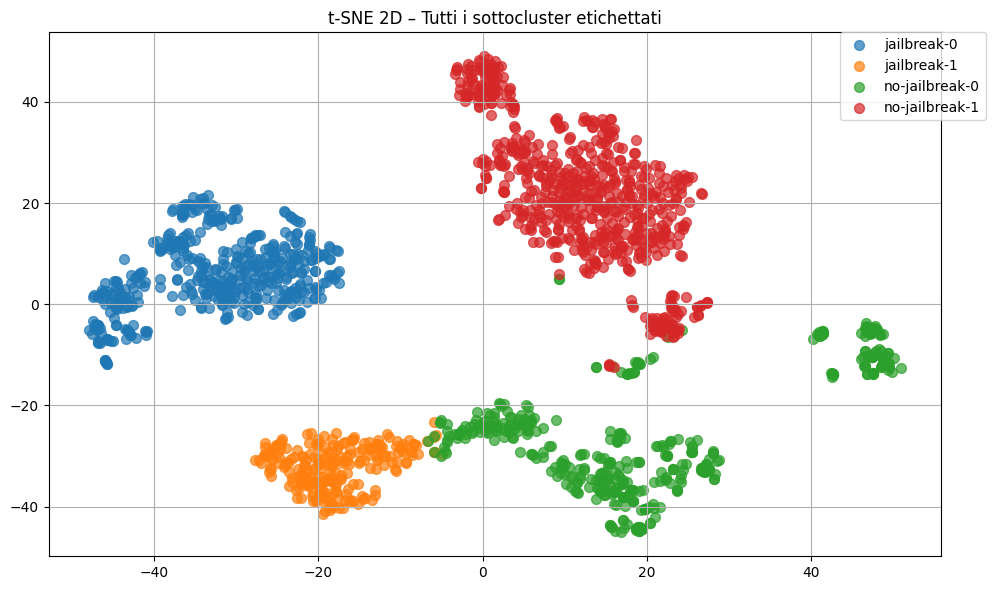
\includegraphics[width=\textwidth]{tsnediv.png}
    \caption{Visualizzazione globale t-SNE con sotto-cluster. La proiezione t-SNE conferma la separazione semantica tra le quattro categorie finali identificate dal clustering gerarchico.}
    \label{fig:global_tsne}
\end{figure}

\subsection{Analisi Dettagliata dei Sotto-Cluster}

\subsubsection{Sotto-Cluster No-Jailbreak}

Le Figure \ref{fig:nojail_pca} e \ref{fig:nojail_tsne} mostrano il dettaglio del clustering interno:

\begin{figure}[H]
    \centering
    \begin{subfigure}[b]{0.48\textwidth}
        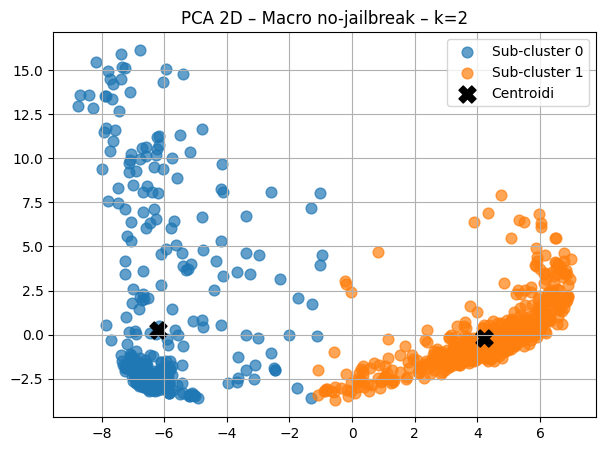
\includegraphics[width=\textwidth]{pca0.png}
        \caption{Proiezione PCA}
        \label{fig:nojail_pca}
    \end{subfigure}
    \hfill
    \begin{subfigure}[b]{0.48\textwidth}
        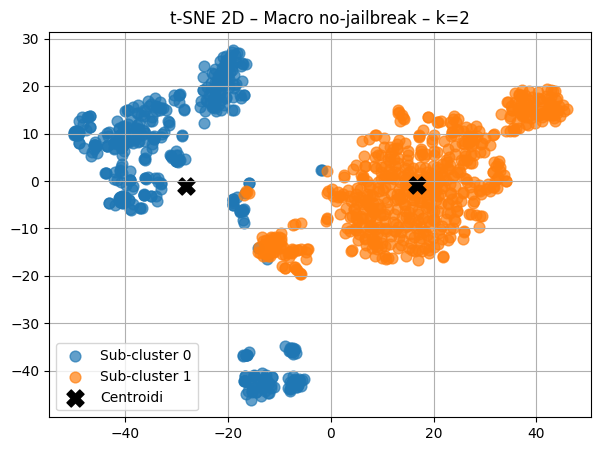
\includegraphics[width=\textwidth]{tsne0.png}
        \caption{Proiezione t-SNE}
        \label{fig:nojail_tsne}
    \end{subfigure}
    \caption{Dettaglio del sotto-clustering per il macro-cluster no-jailbreak (k=2). Il sotto-cluster 0 (blu) rappresenta risposte completamente conformi, mentre il sotto-cluster 1 (arancione) include risposte parzialmente evasive ma accettabili.}
    \label{fig:nojailbreak_detail}
\end{figure}

\subsubsection{Sotto-Cluster Jailbreak}

Le Figure \ref{fig:jail_pca} e \ref{fig:jail_tsne} illustrano la struttura interna del gruppo jailbreak:

\begin{figure}[H]
    \centering
    \begin{subfigure}[b]{0.48\textwidth}
        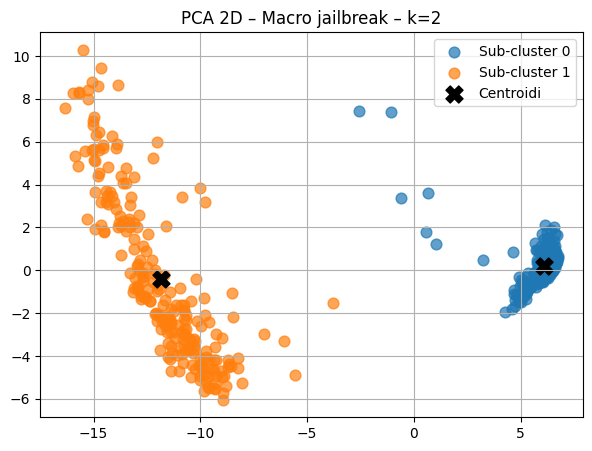
\includegraphics[width=\textwidth]{pca1.png}
        \caption{Proiezione PCA}
        \label{fig:jail_pca}
    \end{subfigure}
    \hfill
    \begin{subfigure}[b]{0.48\textwidth}
        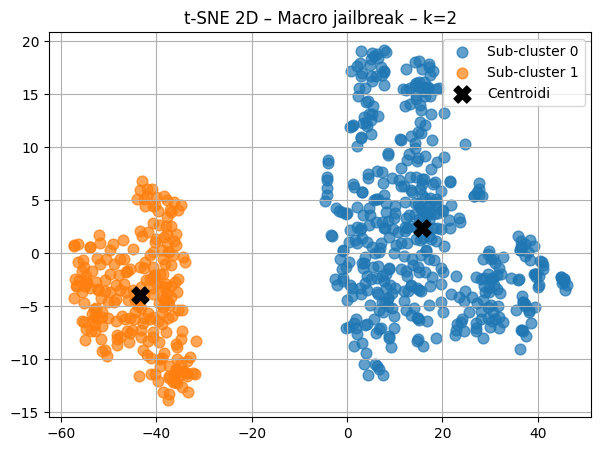
\includegraphics[width=\textwidth]{tsne1.png}
        \caption{Proiezione t-SNE}
        \label{fig:jail_tsne}
    \end{subfigure}
    \caption{Dettaglio del sotto-clustering per il macro-cluster jailbreak (k=2). La separazione netta tra i due sotto-cluster suggerisce tipologie distinte di attacchi jailbreak: diretti/espliciti (cluster 0) e sofisticati/impliciti (cluster 1).}
    \label{fig:jailbreak_detail}
\end{figure}

\section{Discussione Tecnica}

\subsection{Validità della Struttura Gerarchica}

I risultati confermano l'efficacia dell'approccio gerarchico:
\begin{itemize}
    \item \textbf{Silhouette Scores elevati} indicano cluster ben definiti
    \item \textbf{Coerenza semantica} tra le categorie identificate
    \item \textbf{Convergenza multi-tecnica} delle visualizzazioni (PCA, t-SNE, UMAP)
    \item \textbf{Scalabilità} dell'approccio per dataset più ampi
\end{itemize}

\subsection{Interpretazione dei Pattern Identificati}

La struttura finale rivela quattro categorie semanticamente coerenti:
\begin{enumerate}
    \item \textbf{no-jailbreak-0}: Risposte completamente conformi (maggioranza del cluster blu)
    \item \textbf{no-jailbreak-1}: Risposte evasive ma accettabili (cluster rosso)
    \item \textbf{jailbreak-0}: Jailbreak espliciti e diretti (cluster blu nel gruppo jailbreak)
    \item \textbf{jailbreak-1}: Jailbreak sofisticati o impliciti (cluster arancione)
\end{enumerate}

\subsection{Implicazioni per la Sicurezza AI}

L'identificazione automatica di sotto-pattern offre:
\begin{itemize}
    \item \textbf{Granularità aumentata} nella classificazione di sicurezza
    \item \textbf{Identificazione proattiva} di nuove tipologie di attacco
    \item \textbf{Calibrazione migliorata} dei sistemi di filtro
    \item \textbf{Monitoraggio continuo} dell'evoluzione delle tecniche di jailbreak
\end{itemize}

\section{Metriche di Valutazione}

\begin{table}[H]
\centering
\begin{tabular}{lcc}
\toprule
\textbf{Metrica} & \textbf{Macro-Cluster 0} & \textbf{Macro-Cluster 1} \\
\midrule
Silhouette Score & 0.438 & 0.655 \\
Elementi & 1,087 & 686 \\
K ottimale & 2 & 2 \\
Inertia iniziale & $\sim$41,000 & $\sim$23,500 \\
Inertia finale & $\sim$25,000 & $\sim$19,500 \\
Riduzione inertia & 39.0\% & 17.0\% \\
\bottomrule
\end{tabular}
\caption{Metriche comparative dei macro-cluster}
\label{tab:metrics}
\end{table}

\section{Limitazioni e Considerazioni}

\textbf{Limitazioni identificate:}
\begin{itemize}
    \item Dipendenza dalla qualità degli embeddings iniziali
    \item Sensibilità ai parametri di clustering
    \item Necessità di validazione qualitativa delle categorie
\end{itemize}

\textbf{Considerazioni metodologiche:}
\begin{itemize}
    \item L'approccio non supervisionato elimina bias di labeling
    \item La struttura gerarchica mantiene interpretabilità
    \item La scalabilità è garantita dalla complessità computazionale lineare
\end{itemize}

\section{Conclusioni}

Lo studio dimostra l'efficacia del clustering gerarchico nell'identificazione automatica di pattern jailbreak in risposte generate. I risultati principali includono:

\begin{enumerate}
    \item \textbf{Separazione efficace} tra jailbreak e no-jailbreak con accuratezza strutturale elevata
    \item \textbf{Identificazione} di quattro sotto-categorie semanticamente coerenti
    \item \textbf{Validazione} attraverso multiple tecniche di riduzione dimensionale
    \item \textbf{Applicabilità pratica} per sistemi di sicurezza AI in produzione
\end{enumerate}

\subsection{Contributi Originali}

\begin{itemize}
    \item Metodologia gerarchica a due livelli per classificazione jailbreak
    \item Ottimizzazione automatica del numero di cluster tramite Silhouette Analysis
    \item Validazione multi-tecnica della struttura cluster identificata
    \item Framework scalabile per l'analisi di sicurezza AI
\end{itemize}

\subsection{Sviluppi Futuri}

Le direzioni di ricerca future includono:
\begin{itemize}
    \item Estensione a dataset multi-linguistici
    \item Integrazione con tecniche di deep clustering
    \item Sviluppo di metriche di sicurezza personalizzate
    \item Implementazione in sistemi di monitoring real-time
\end{itemize}

\section*{Ringraziamenti}

Si ringrazia per il dataset fornito e per il supporto computazionale che ha reso possibile questa analisi sperimentale.

\end{document}